%!TEX root = skripsi.tex
%-----------------------------------------------------------------------------%
\chapter{\babSatu}
%-----------------------------------------------------------------------------%


%-----------------------------------------------------------------------------%
\section{Latar Belakang}
%-----------------------------------------------------------------------------%
	
	Saat ini, perkembangan teknologi semakin mempermudah berbagai kegiatan manusia yang dilakukan sehari-hari. Sebagai contoh, ketika seseorang mengalami permasalahan kesehatan dan ingin berkonsultasi kepada para dokter, ia dapat memanfaatkan forum kesehatan \textit{online} yang dapat memungkinkan terjadinya interaksi antara pasien dan dokter tanpa perlu tatap muka.  Melalui forum tersebut, seseorang hanya perlu menuliskan keluhan dan pertanyaan pada formulir yang tersedia. Kemudian, dokter yang memiliki akun di forum kesehatan \textit{online} tersebut dapat memberikan jawaban atas pertanyaan orang tersebut.
	
	Banyak sekali informasi bermanfaat yang dapat diperoleh dari forum kesehatan \textit{online}. Informasi tersebut meliputi informasi keluhan yang dialami pasien, obat yang sebaiknya digunakan atau langkah penyembuhan yang dapat dilakukan. Orang lain dapat mencari obat atau langkah penyembuhan dari forum tersebut melalui pertanyaan yang sudah diajukan sebelumnya. Oleh karena itu, akan sangat baik apabila ada sebuah model atau sistem yang mampu mengekstrak secara otomatis informasi-informasi tersebut. Tantangan utama dari pengembangan model ini adalah \textit{post} atau isi dari forum yang tidak terstruktur. Dokumen \textit{post} tidak dibagi menjadi beberapa bagian seperti bagian keluhan, penyakit, obat dan lain sebagainya, namun hanya menjadi satu bagian saja. Misalnya ketika seseorang menanyakan tentang keluhannya, orang tersebut hanya diberikan dua buah isian berupa judul dan isi pertanyaan. Jawaban yang diberikan oleh dokter juga sama, hanya menjadi satu bagian saja. Jawaban yang diberikan tidak terstruktur seperti memiliki bagian langkah penyembuhan, nama penyakit dan obat secara terpisah. Hal ini menyebabkan orang sulit melakukan ekstraksi informasi dari dokumen tersebut.
	
	Dari permasalahan tersebut, terdapat sebuah solusi untuk melakukan ekstraksi informasi penyakit dalam suatu dokumen, yaitu dengan menggunakan sistem Pengenalan Entitas Kesehatan (\textit{Medical Entity Recognition}) atau disingkat MER. Sistem \mer~ini dapat mengenali entitas kesehatan dalam sebuah dokumen. Apabila diberikan sebuah dokumen, sistem ini akan mengembalikan dokumen yang telah mendapatkan label pada masing-masing entitas kesehatan di dalamnya.
	
	Penelitian dalam rangka mengembangkan sistem \mer~sudah banyak dilakukan oleh beberapa peneliti. Salah satu penelitian tersebut dilakukan oleh \cite{abacha2011medical} dengan menggunakan dokumen medis rumah sakit berbahasa Inggris. Entitas yang mendapatkan label pada penelitian tersebut adalah \textit{treatment}, \textit{problem} dan \textit{test}. Terdapat tiga pendekatan yang digunakan, yaitu pendekatan \textit{machine learning}, pendekatan \textit{rule based} dan pendekatan \textit{hybrid}. Kesimpulan yang dicapai pada penelitian tersebut adalah pendekatan \textit{hybrid} memberikan hasil terbaik, yaitu dengan \textit{precision} $ 72.18\% $, \textit{recall} $ 83.78\% $ dan \textit{F-Measure} $ 77.55\% $.
		
	Pada dokumen berbahasa Indonesia, pengembangan sistem \mer~masih belum banyak dilakukan. Ada beberapa penelitian terkait sistem \mer, namun hasil yang diberikan belum memuaskan. Salah satu penelitian terkait \mer~dilakukan oleh \cite{skripsiKakRadit} yang menggunakan dokumen forum kesehatan \textit{online} berbahasa Indonesia dari beberapa situs. Tujuan dari penelitian tersebut adalah untuk mencari kombinasi fitur yang dapat menghasilkan akurasi terbaik. \cite{skripsiKakRadit} menggunakan algoritma \textit{Conditional Random Fields} dengan hasil akhir yaitu \textit{precission}~70.97\%, \textit{recall}~57.83\% dan \textit{f-measure}~63.69\%. Fitur-fitur yang membuat model memiliki akurasi terbaik yaitu fitur kata itu sendiri, frasa, kamus: \textit{symptom, disease, treatment, drug}, \textit{window feature (previous word)} dan panjang kata.
	
	Dalam penelitian ini \saya~memandang permasalahan pelabelan dokumen kesehatan sebagai permasalahan \textit{sequence labeling}. Kami mengusulkan penggunaan teknik \textit{Deep Learning} dengan menggunakan \textit{Recurrent Neural Networks} (RNNs), karena RNNs merupakan \textit{state-of-the-art} untuk permasalahan \textit{sequence labeling} seperti permasalahan pada penelitian ini. Sebelumnya penelitian terkait hal ini pernah dikerjakan oleh \cite{mujiono2016new}, dengan jenis entitas yang digunakan adalah entitas \textit{Drug} saja. Peneliti tersebut menggunakan model RNNs untuk melabeli dokumen secara otomatis. Dengan menggunakan fitur vektor kata yang menggunakan \textit{word embedding} saja, \textit{f-measure} yang diberikan mencapai 86.45\%. Oleh karena itu, \saya~mengusulkan model RNNs pada penelitian ini.
		
	\Saya~berharap bahwa penelitian ini akan memberikan banyak manfaat. Sistem \mer~yang dihasilkan dapat digunakan untuk membuat aplikasi lain. Misalnya dengan adanya \mer~pada dokumen bahasa Indonesia, dapat dibuat sistem untuk melakukan \textit{indexing} dokumen forum sehingga pencarian dokumen kesehatan dapat dilakukan dengan lebih efisien. Selain itu, keluaran dari \mer~juga dapat digunakan untuk mengidentifikasi tren penyakit pada waktu tertentu dari suatu sumber, sehingga pihak terkait mampu melakukan langkah dan kebijakan yang tepat. Sistem \mer~juga dapat digunakan pada aplikasi \textit{Question Answering} \citep{abacha2011medical} dengan cara memanfaatkan hasil pelabelan untuk melakukan identifikasi entitas yang ditanyakan. Gambar \ref{fig:merforqa} merupakan contoh penggunaan \mer~pada aplikasi \textit{question answering} dalam bidang kesehatan.
	
	\begin{figure}
		\centering
		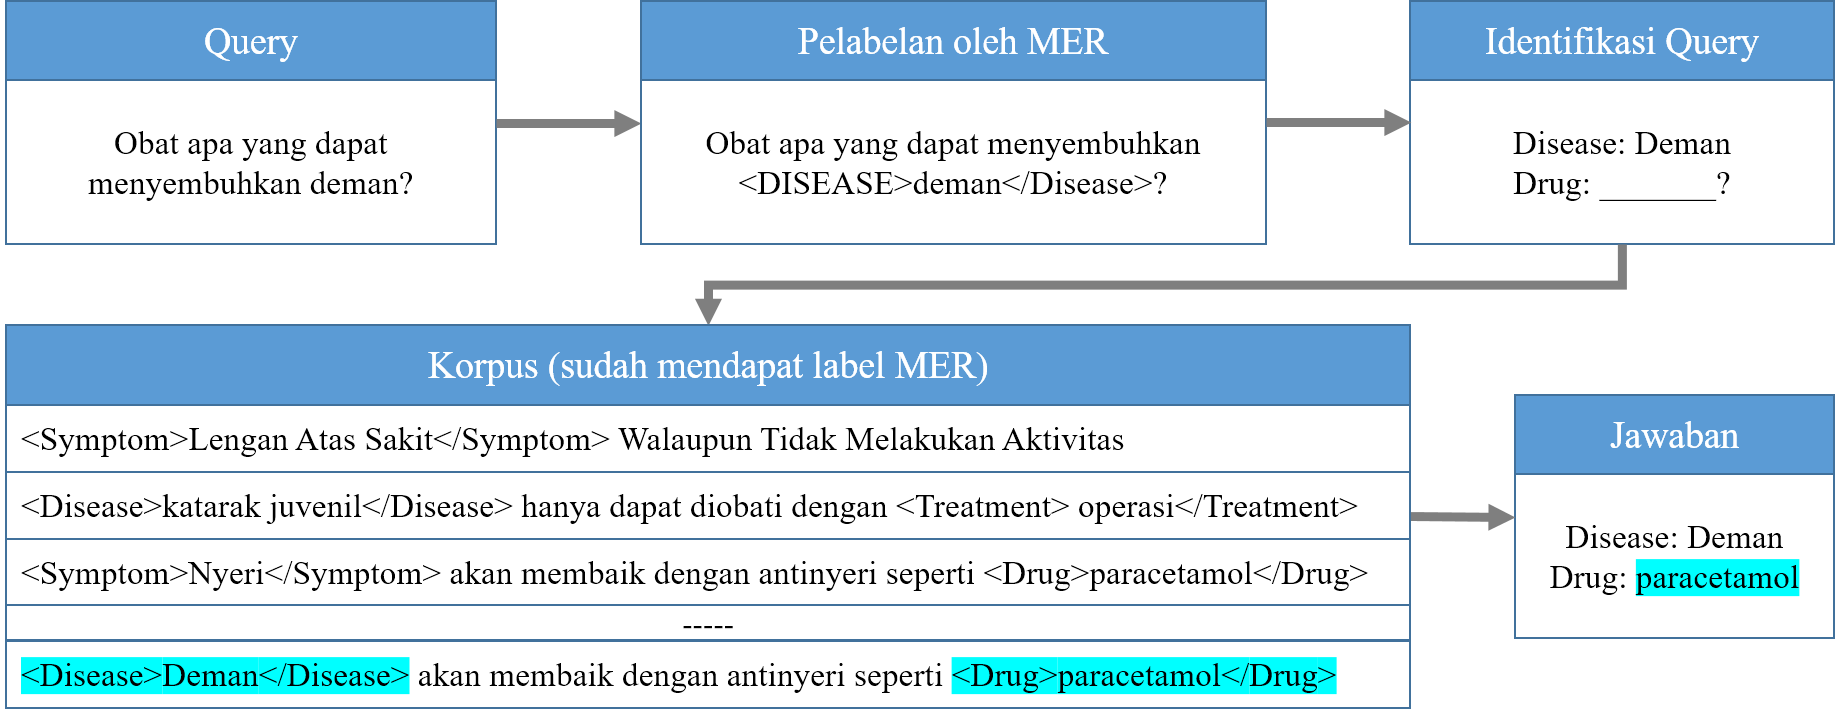
\includegraphics[width=\linewidth]{images/merforqa}
		\caption{Diagram Penggunaan MER pada aplikasi \textit{Question Answering}}
		\label{fig:merforqa}
	\end{figure}
	
	\Saya~berharap bahwa penelitian \mer~pada dokumen berbahasa Indonesia ini dapat dilanjutkan sehingga dapat menghasilkan model yang lebih baik dan membuat suatu aplikasi yang memanfaatkan keluaran dari penelitian ini. Masih banyak manfaat lain yang didapatkan dengan adanya sistem \mer~yang memiliki hasil akurat. 

%-----------------------------------------------------------------------------%
\section{Perumusan Masalah}
%-----------------------------------------------------------------------------%
Berdasarkan latar belakang di atas, dalam penelitian ini \saya~ mengajukan rumusan masalah sebagai berikut:
\begin{enumerate}
	% Bagaimana --- %
	\item Bagaimana performa RNNs dibandingkan dengan CRFs (\textit{baseline}) untuk sistem \mer~yang dikembangkan?
	\item Fitur apa saya yang membuat sistem \mer~memiliki performa terbaik?
\end{enumerate}

%-----------------------------------------------------------------------------%
\section{Tujuan dan Manfaat Penelitian}
%-----------------------------------------------------------------------------%
Penelitian ini bertujuan untuk membangun sistem yang mampu melakukan ekstraksi entitas kesehatan dari forum \textit{online}. Sebenarnya, pada penelitan yang dilakukan oleh \cite{skripsiKakRadit} sudah menghasilkan sebuah sistem yang sama. Namun, fokus penelitian ini yaitu mencoba menggunakan metode yang berbeda. Metode tersebut yaitu dengan menggunakan RNNs dengan harapan mampu memberikan hasil yang lebih baik. Penelitian ini juga bertujuan untuk mendapatkan fitur-fitur yang membuat sistem memiliki performa terbaik. Selain itu, penelitian ini juga bertujuan untuk mendapatkan informasi baru terkait pembuatan sistem \mer~berbahasa Indonesia.

Manfaat dari penelitian ini adalah menghasilkan rancangan sistem dan metode yang dapat digunakan sebagai bahan penelitian lanjutan. Saat ini, sistem dan metode yang dihasilkan hanya mampu mengenali entitas kesehatan saja. Hal ini dapat digunakan untuk membuat sistem informasi tentang suatu jenis penyakit lengkap dengan gejala, obat dan cara penyembuhannya. Selama ini, masyarakat yang menanyakan suatu penyakit melalui forum \ol~tidak membaca terlebih dahulu riwayat pertanyaan yang telah ditanyakan oleh orang lain. Oleh karena itu, diharapkan dengan sistem informasi tersebut, calon penanya hanya perlu mencari penyakit yang akan ditanyakan pada sistem informasi tersebut. Apabila tidak ada, penanya dapat mengajukan pertanyaan, kemudian pertanyaan dan jawaban yang diberikan akan terindeks oleh sistem dan menambah informasi. 

Selain itu, hasil penelitian ini juga dapat digunakan untuk membangun sistem yang mengenali tren penyakit pada masyarakat, sehingga pihak terkait mampu menentukan langkah strategis yang tepat. Sistem \mer~juga dapat digunakan pada aplikasi \textit{Question Answering} \citep{abacha2011medical} dengan cara memanfaatkan hasil pelabelan untuk melakukan identifikasi entitas yang ditanyakan.

%-----------------------------------------------------------------------------%
\section{Metodologi Penelitian}
%-----------------------------------------------------------------------------%
Berikut merupakan metode penelitian yang \saya~lakukan.
\begin{enumerate}
	\item Studi Literatur\\
	Pada tahapan ini \saya~mencari literatur yang terkait dengan penelitian ini. Literatur ini digunakan sebagai bahan pemelajaran dan untuk mendukung penelitian yang \saya~lakukan. Literatur yang \saya~gunakan memiliki keterkaitan terhadap kasus \mer, \textit{Sequence Labeling} dan \rnn.
	
	\item Pengumpulan Data \\
	Pada tahapan ini, \saya~mengumpulkan data percobaan yang diperlukan. \Saya~mengumpulkan dokumen teks dari forum kesehatan \textit{online} dan dari penelitian \cite{skripsiKakRadit}. Setelah dokumen terkumpul, \saya~melakukan langkah-langkah pra-pemrosesan baik pada dokumen yang \saya~dapatkan dari forum maupun korpus dari penelitian \cite{skripsiKakRadit}. Tujuan langkah tersebut yaitu untuk menghilangkan beberapa karakter yang mengganggu tahapan selanjutnya, melakukan normalisasi pada beberapa kasus token, dan lain sebagainya. Setelah itu \saya~melakukan tokenisasi dan melakukan pemecahan kalimat dengan menggunakan beberapa aturan, kemudian \saya~memberikan label pada dokumen yang \saya~dapat dari forum secara manual. 
	
	\item Pengembangan Model\\
	Pada tahapan ini, \saya~melakukan perancangan eksperimen yang akan dilakukan. \Saya~mendefinisikan fitur-fitur yang akan diuji pada penelitian ini dan arsitektur RNNs yang juga akan diuji.
		
	\item Eksperimen \\
	Tahapan ini merupakan bagian inti dari penelitian. \saya~melakukan langkah eksperimen dengan tujuan mendapatkan jawaban dari pertanyaan yang telah dirumuskan pada rumusan masalah. Sebelum masuk di tahap ini, \saya~melakukan pemecahan data menjadi 10 bagian untuk mengimplementasikan \textit{10-cross fold validation}. Setelah itu, data disusun sedemikian sehingga siap digunakan sebagai \textit{resource} eksperimen.
	
	\item Evaluasi dan Analisis Hasil \\
	Pada tahapan ini \saya~melakukan evaluasi dan analisis dari hasil eksperimen. Untuk mengukur akurasi dari masing-masing fitur dan arsitektur RNNs yang \saya~usulkan, saya menggunakan \textit{precision}, \textit{recall} dan \textit{f-measure}.
		
	\item Penarikan Kesimpulan \\
	Tahap ini merupakan tahap terakhir dari penelitian. Setelah melakukan serangkaian eksperimen, evaluasi dan analisis, \saya~memberikan kesimpulan dan informasi penting terkait penelitian ini. Selain itu \saya~juga memberikan saran untuk penelitian selanjutnya.
\end{enumerate}

%-----------------------------------------------------------------------------%
\section{Ruang Lingkup Penelitian}
Pada penelitian ini terdapat beberapa batasan yang \saya~tentukan, yaitu:
\begin{enumerate}
\item{\bf Entitas Kesehatan}\\
Pengenalan entitas kesehatan pada penelitian ini berfokus pada pengenalan nama penyakit (\disease), gejala-gejala penyakit (\symptom), nama obat (\drug) dan langkah pengobatan (\treatment),

\item{\bf Domain Pengenalan}\\
Pengenalan entitas kesehatan dilakukan pada bagian judul pertanyaan, isi pertanyaan/keluhan dan isi jawaban dari dokter.
\end{enumerate}

%-----------------------------------------------------------------------------%

%-----------------------------------------------------------------------------%
\section{Sistematika Penulisan}
%-----------------------------------------------------------------------------%
Sistematika penulisan dalam laporan penelitian ini sebagai berikut:
\begin{itemize}

	\item Bab 1 \babSatu \\
	Pada bab ini \saya~menjelaskan mengenai motivasi dalam melakukan penelitian ini dan komponen-komponen utama penelitian seperi latar belakang, perumusan masalah, tujuan dan manfaat penelitian, metodologi penelitian, ruang lingkup penelitian dan sistematika penulisan.
	
	\item Bab 2 \babDua \\
	Pada bab ini \saya~melakukan studi literatur mengenai beberapa teori dan penelitian yang dilakukan oleh penulis lain. 
		
	\item Bab 3 \babTiga \\
	Pada bab ini \saya~menjelaskan alur dari penelitian ini, yaitu pengumpulan data, pra-pemrosesan, pelabelan, pengembangan model, eksperimen dan evaluasi.
		
	\item Bab 4 \babEmpat \\
	Pada bab ini \saya~menjelaskan proses implementasi sistem dan eksperimen berdasarkan rancangan yang telah \penulis~tentukan pada bab sebelumnya. Selain itu \saya~juga menjelaskan implementasi dari masing-masing tahapan yang dilakukan.
		
	\item Bab 5 \babLima \\
	Pada bab ini \saya~menjelaskan analisis dari hasil eksperimen yang telah \saya~kerjakan pada tahap sebelumnya. Hasil eksperimen \saya~sajikan dalam bentuk tabel dan grafik.
	
	\item Bab 6 \babEnam \\
	Pada bab ini \saya~memberikan kesimpulan berdasarkan hasil eksperimen dan analisis yang telah dilakukan pada penelitian ini. Selain itu \saya~juga memberikan saran dan masukan untuk penelitian dan pengembangan sistem mengenai \mer~berbahasa Indonesia selanjutnya.
	
\end{itemize}